\chapter{Release 1: Users, segmentation \& channels}

\phantomsection
\section*{Introduction}
In this chapter, we focus on the first release of our product, this release aims to create and enhance
the user experience, implement userbase segmentation strategies, and manage notification channels.
We will delve into the sprints backlog, design considerations, and the implementation process
undertaken to bring these features to fruition.

\addcontentsline{toc}{section}{Introduction}

\section{Sprints backlog}
During the Sprint Planning event, we estimated the effort required for each item in the sprint backlog
based on the number of working hours.

The priority of backlog items is reflected by their relative order in the table. Items positioned
higher in the table indicate a higher priority. \\

\begin{longtable}{ | m{0.08\textwidth}  | m{0.17\textwidth} | m{0.48\textwidth} | c | }
    \hline
    \textbf{Sprint}         & \textbf{Epic}                                       & \textbf{User story}                                                                                                                   & \textbf{Estimation} \\
    \hline
    \endfirsthead
    \hline
    \textbf{Sprint}         & \textbf{Epic}                                       & \textbf{User story}                                                                                                                   & \textbf{Estimation} \\
    \hline
    \endhead
    \hline
    \endfoot
    \endlastfoot
    \multirow[t]{3}{5em}{1} & \multirow{2}{5em}{Authentication}                   & As a new user, I want to be able to create an account so that I can use the notification center.                                      & 16                  \\
    \cline{3-4}
                            &                                                     & As a registered user, I want to be able to log into my account securely using my email and password.                                  & 16                  \\
    \cline{2-4}
                            & \multirow{4}{5em}{Agents management}                & As an administrator, I want to be able to create agents so that I can add them to the notification center.                            & 16                  \\
    \cline{3-4}
                            &                                                     & As an administrator, I want to be able to list agents so that I can view all registered agents.                                       & 16                  \\
    \cline{3-4}
                            &                                                     & As an administrator, I want to be able to edit agents so that I can modify their information.                                         & 8                   \\
    \cline{3-4}
                            &                                                     & As an administrator, I want to be able to delete agents so that I can get rid of no longer needed agents.                             & 8                   \\
    \cline{2-4}
                            & \multirow{4}{5em}{Users management}                 & As an administrator/agent, I want to be able to create users so that I can send them notifications.                                   & 16                  \\
    \cline{3-4}
                            &                                                     & As an administrator/agent, I want to be able to list users so that I can view all created users.                                      & 16                  \\
    \cline{3-4}
                            &                                                     & As an administrator/agent, I want to be able to edit users so that I can modify their information.                                    & 8                   \\
    \cline{3-4}
                            &                                                     & As an administrator/agent, I want to be able to delete users so that I can get rid of no longer needed users.                         & 8                   \\
    \hline
    \multirow[t]{2}{5em}{2} & \multirow{4}{5em}{Audience management}              & As an administrator/agent, I want to be able to create an audience so that I can target specific individuals based on a criteria.     & 24                  \\
    \cline{3-4}
                            &                                                     & As an administrator/agent, I want to be able to list audiences so that I can view all created segments.                               & 16                  \\
    \cline{3-4}
                            &                                                     & As an administrator/agent, I want to be able to edit an audience so that I can change selection criteria and segment configurations.  & 8                   \\
    \cline{3-4}
                            &                                                     & As an administrator/agent, I want to be able to delete a group of users so that I can get rid of no longer needed groups..            & 8                   \\
    \cline{2-4}
                            & \multirow{4}{5em}{Notification channels management} & As an administrator/agent, I want to be able to create notification channels so that I can send notifications through these channels. & 32                  \\
    \cline{3-4}
                            &                                                     & As an administrator/agent, I want to be able to list notification channels so that I can view all created channels.                   & 16                  \\
    \cline{3-4}
                            &                                                     & As an administrator, I want to be able to edit notification channels so that I can modify or update their configurations.             & 8                   \\
    \cline{3-4}
                            &                                                     & As an administrator/agent, I want to be able to delete notification channels so that I can get rid of no longer used channels.        & 8                   \\
    \hline
    \caption{Backlog of Sprint 1 \& 2}
\end{longtable}

\section{Design}
The design phase of software development is a critical step in the software development life cycle.
It is the process of transforming the customer requirements into a detailed plan for how the software
will be implemented. In this section we are going to focus on the design aspects related to the software
and database design.

\subsection{Class diagram}
The class diagram provides a high-level overview of the system's structure, relationships,
and interactions between different classes. It represents the static structure of the system,
including classes, attributes, methods, and associations.

The figure \ref{g-class} illustrates the class diagram for our first release.

\begin{figure}[hbt!]
    \centering
    \includesvg[width=\textwidth]{diagrams/class/r1-class}
    \caption{Notification Center global class diagram}
    \label{g-class}
\end{figure}

\subsection{Database design}
The figure \ref{g-erd}  illustrates the entity-relationship diagram for our first release.

\begin{landscape}
    \begin{figure}[hbt!]
        \centering
        \includesvg[width=1.55\textwidth]{diagrams/database/erd}
        \caption{Notification Center Entity-Relationship diagram}
        \label{g-erd}
    \end{figure}
\end{landscape}


\subsection{Sequence diagrams}
\subsubsection{Sequence diagram for Creating a Channel}


\begin{landscape}
    \begin{figure}[hbt!]
        \centering
        \includesvg[width=1.55\textwidth]{diagrams/sequence/seq-create-channel}
        \caption{Sequence diagram for Creating a Channel}
        \label{seq-create-channel}
    \end{figure}
\end{landscape}



\section{Implementation}
\subsection{Authentication page}
The figure \ref{ss-signin} illustrates the final result of the implementation of the authentication epic.
\begin{figure}[hbt!]
    \centering
    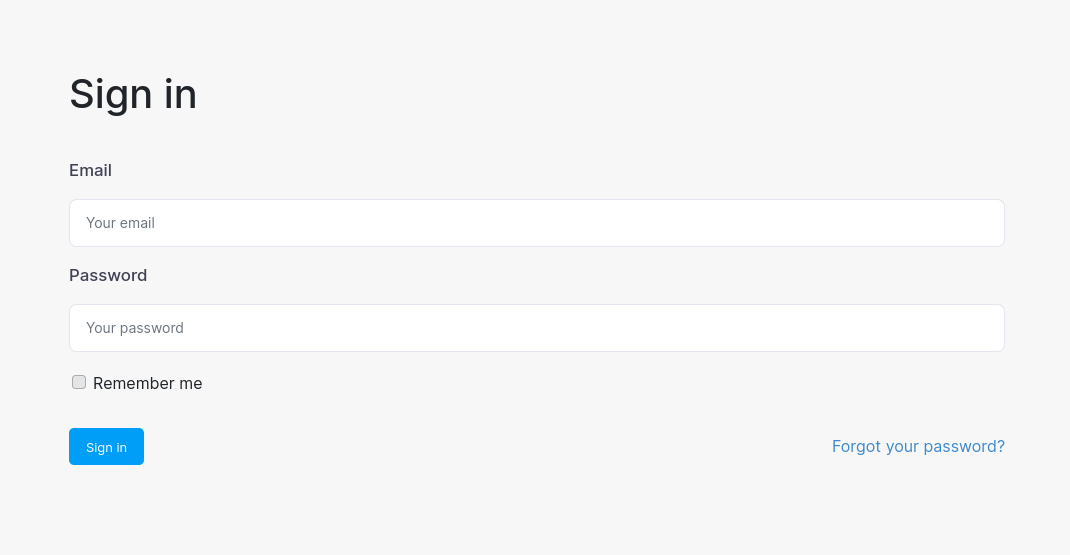
\includegraphics[width=\textwidth]{app/signin}
    \caption{Authentication page}
    \label{ss-signin}
\end{figure}

\subsection{Agents management page}
The figure \ref{ss-agents} illustrates the final result of the implementation of the agents management epic.
\begin{figure}[hbt!]
    \centering
    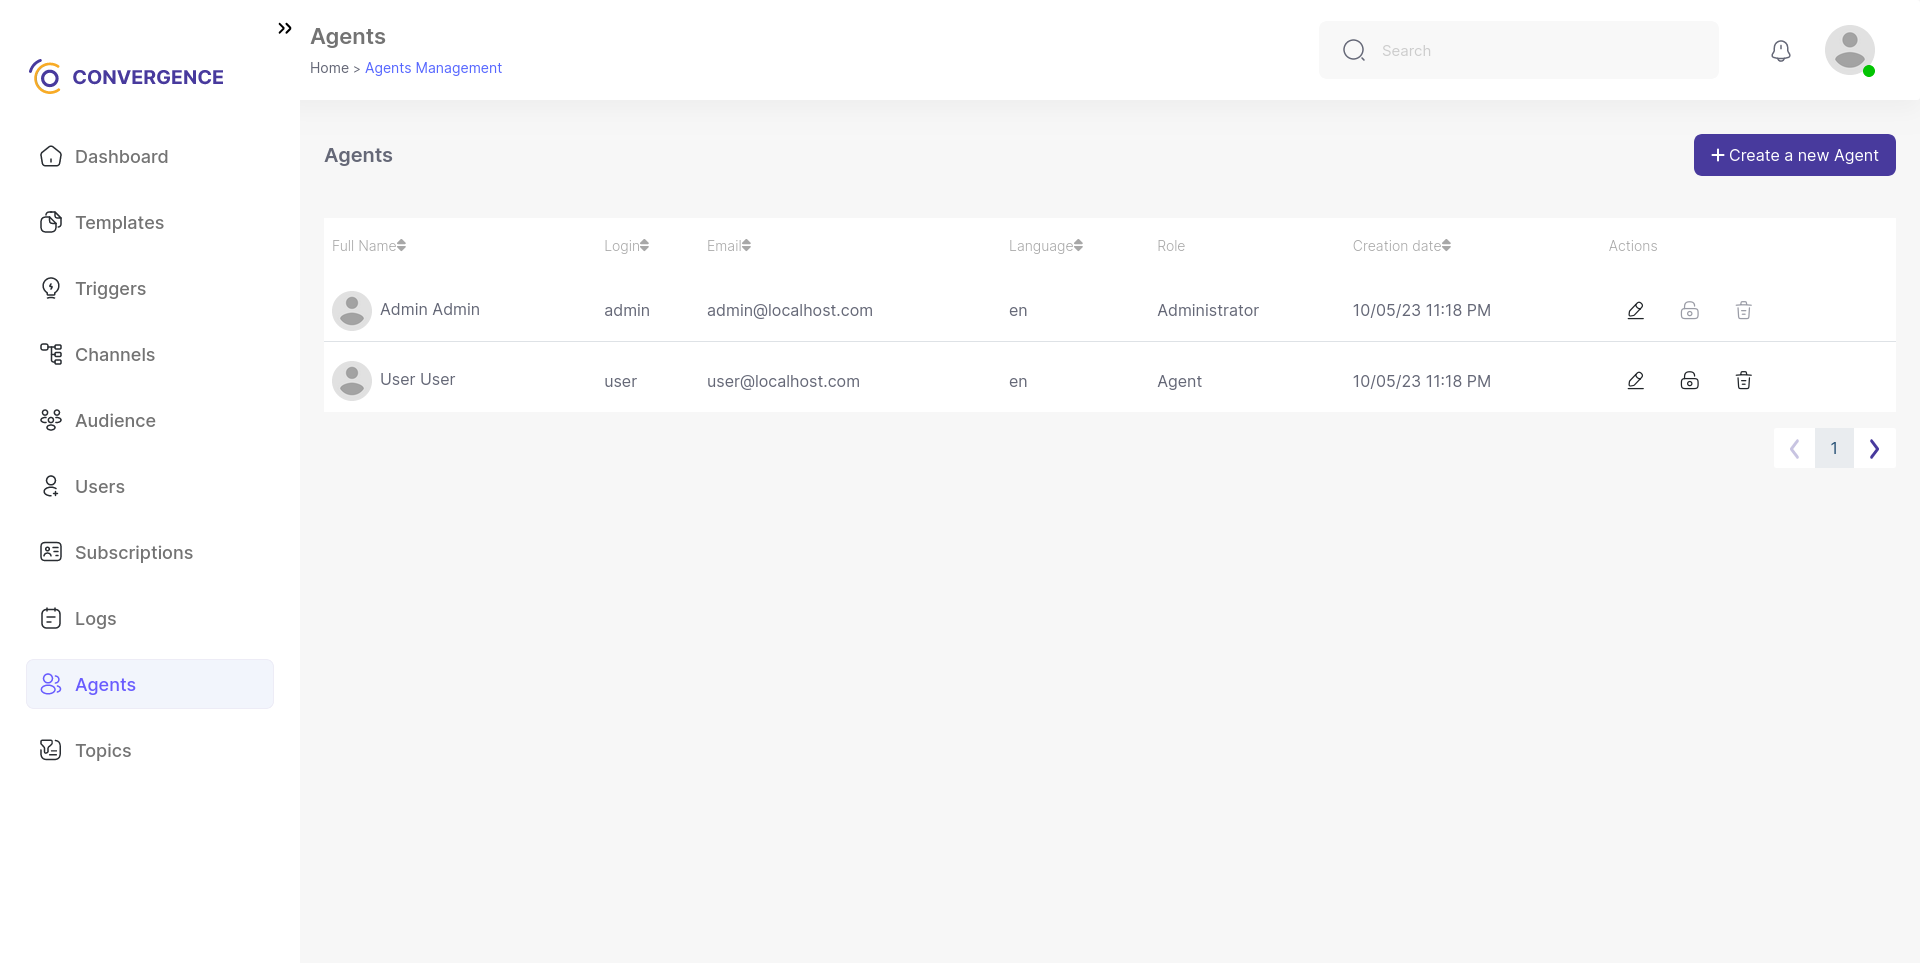
\includegraphics[width=\textwidth]{app/agents}
    \caption{Agents management page}
    \label{ss-agents}
\end{figure}

\subsection{Channels management page}
The figure \ref{ss-channels} illustrates the final result of the implementation of the channels management epic.
\begin{figure}[hbt!]
    \centering
    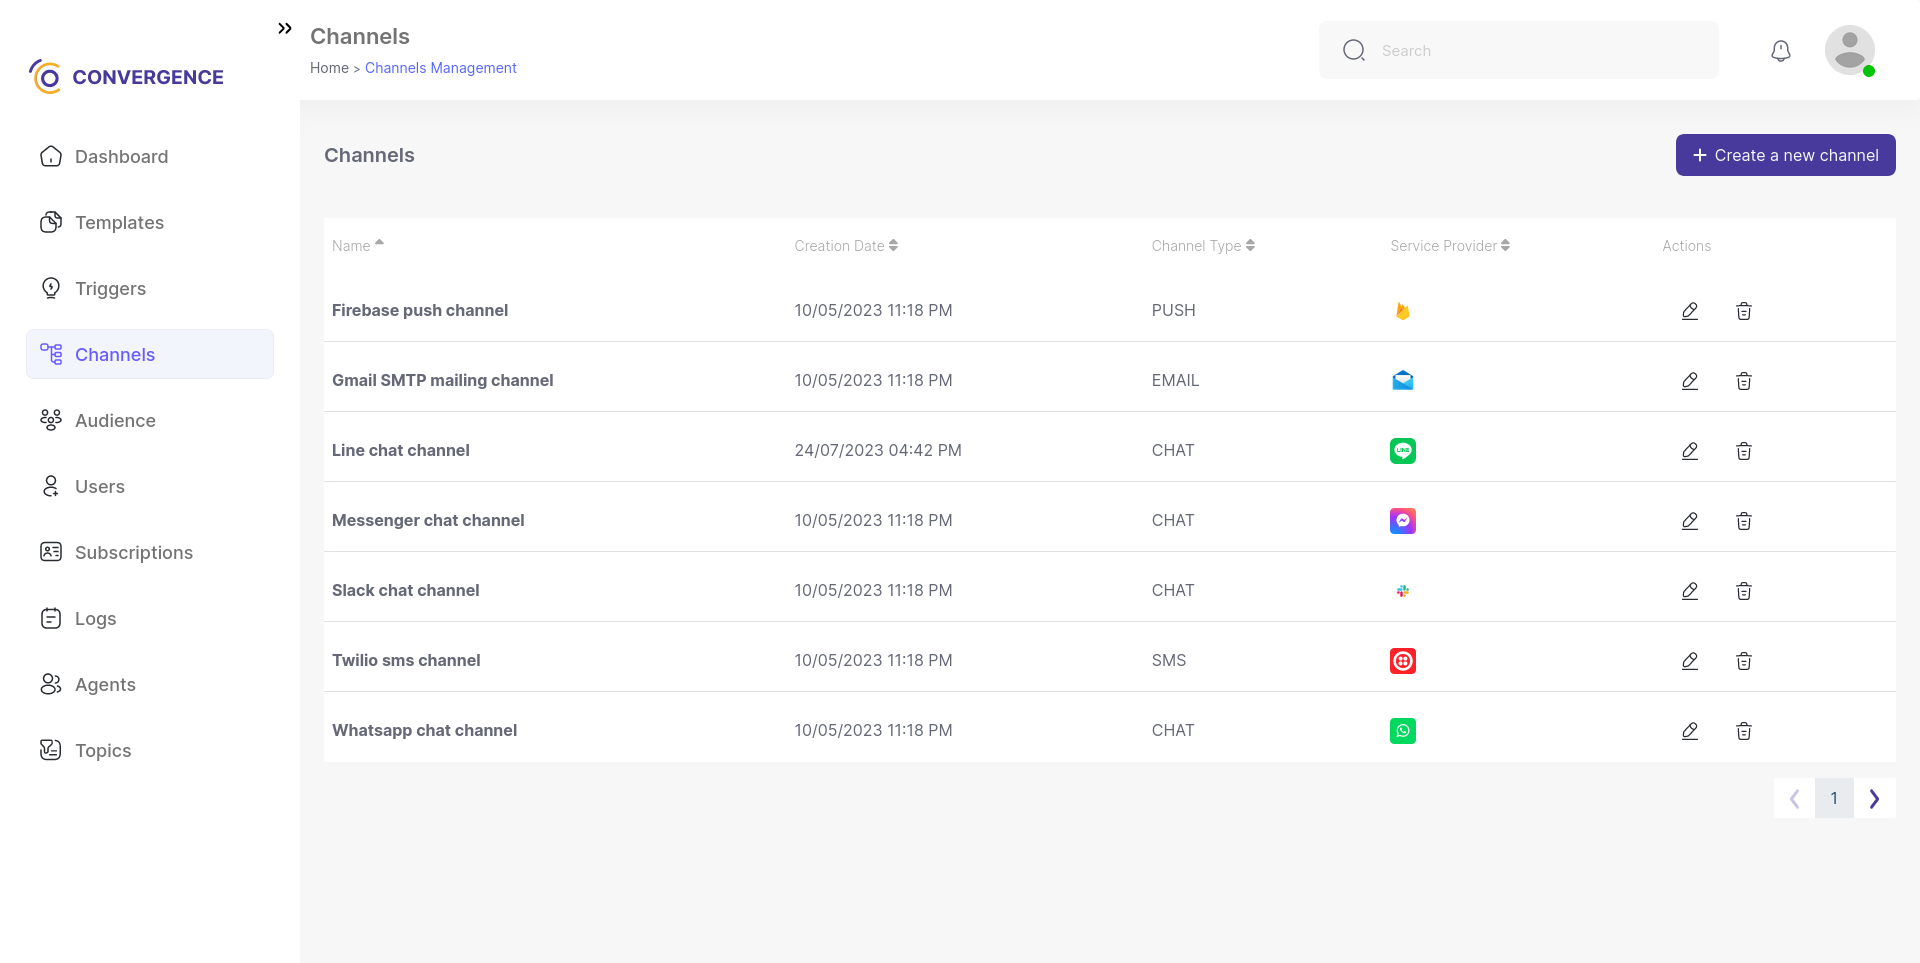
\includegraphics[width=\textwidth]{app/channels}
    \caption{Channels management page}
    \label{ss-channels}
\end{figure}

\phantomsection
\section*{Summary}
\addcontentsline{toc}{section}{Summary}